% \documentclass{article}
% \usepackage[utf8]{inputenc}
\documentclass{assignment format}
\usepackage{assignment}
\usepackage{bm}
\setcounter{section}{-1}
\setcounter{subsection}{-1}
\usepackage{kotex}

\usepackage{amsmath, amsthm, amssymb}
\usepackage{enumerate}
\usepackage{enumitem}
\usepackage{kotex}
\usepackage{amsfonts}
\usepackage[dvipsnames]{xcolor}
\usepackage{enumitem}
\usepackage{url}
\usepackage{graphicx}
\usepackage{float} 
\usepackage{physics}
\usepackage{bbm}
\usepackage{caption}
\usepackage{minted}
\usepackage{todonotes}
\usepackage{relsize}
\usepackage{float}
\usepackage{blindtext}
\usepackage{multicol}
\newcommand{\note}[4][]{\todo[author=#2,color=#3,size=\scriptsize,fancyline,caption={},#1]{#4}} % default note settings, used by macros below.
\newcommand{\mrinmaya}[2][]{\note[#1]{mrinmaya}{blue!40}{#2}}

\usepackage[colorlinks=true]{hyperref}

\DeclareMathOperator*{\argmax}{arg\,max}

\newenvironment{answer}{
    {\bf Answer:} \begingroup\color{red}
}{\endgroup}%

\begin{document}

\makeheader{\textbf{Due on} Friday Nov. 15, 2024 \\ by \textbf{23:59pm}}{Assignment 4: Pre-trained models}
\begin{center}
%%%%%YOUR NAME HERE%%%%%

\fbox{%
  \parbox{\textwidth}{
  \begin{center}
\large\textbf{Honor Pledge for Graded Assignments}
\\ 
\\ 
   \large{ “I, YOUR NAME HERE , affirm that I have not given or received any unauthorized help on this assignment, and that this work is my own.”}
    \end{center}
}%
}
\end{center}

\section{Instructions}
\begin{itemize}
\item Total score cannot exceed 100 points. For example, if you score 95 points from non-bonus questions and 10 points are added from bonus questions, your score will be 100 points, not 105 points.
\item Skeleton codes for each of the problems are at the directory \texttt{/q1} and \texttt{/q2}.  
\item Run the \texttt{bash collect\_submission.sh} script to produce your 2000\_00000\_coding.zip file. Please make sure to modify collect\_sumbssion.sh file before running this command. (\textbf{2000\_00000} stands for your student id)
\item Modify this tex file into \texttt{2000\_00000\_written.pdf} with your written solutions
\item Upload both \texttt{2000\_00000\_coding.zip} and \texttt{2000\_00000\_written.pdf} to etl website. \textbf{(4pts)}
\item \textbf{If submission instructions are not followed, \texttt{4 points} will be deducted.}
\end{itemize}

%%%NOTE FOR MYSELF%%%

\section{Utilizing pre-trained models (50 pts)}
We learned how different pre-trained models work in class. In this assignment, we will load pre-trained models from Hugging Face, and use them for downstream tasks. Please complete the given jupyter notebook files \textbf{(q1/q1a.ipynb)} and \textbf{(q1/q1b.ipynb)}, and submit it along with your answer to this latex file.


\subsection{Inference using a pre-trained Question Answering model (20 pts)}
In this problem, we will utilize a pre-trained BERT(Bidirectional Encoder Representations from Transformers) model for question answering. BERT excels in this task by leveraging its contextual understanding of language, employing techniques such as tokenization, segment embeddings, positional embeddings, and multi-head self-attention to capture intricate relationships between words. During the inference phase, the model predicts answer spans in a passage based on its extensive pre-trained knowledge and fine-tuned task-specific understanding. 

\begin{figure}[h]
    \centering
    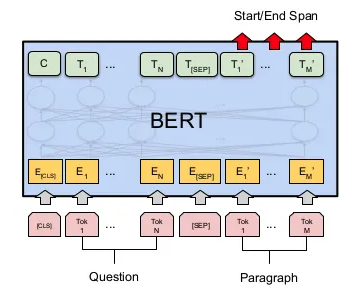
\includegraphics[width=0.4\textwidth]{bert_qa.png}
    \caption{Question answering using BERT}
    \label{fig:word2vec}
\end{figure}

There are various approaches to employing deep learning models for question answering, and we will explore the intricacies of this task in upcoming lectures. For now, prepare for a hands-on journey into loading a pre-trained BERT model from Hugging Face, which encodes questions and context together and answers by selecting a span in the given context. The model's output includes scores for the start and end positions of the answer span. Follow the instructions in the provided Jupyter notebook to complete the code.


\begin{enumerate}[label=(\alph*)]
    \item Load the pre-trained model and tokenizer and complete the \texttt{\_\_init\_\_} function. \textbf{(2 pts)}
    \item Implement the \texttt{tokenize} function to encode the question and context. \textbf{(6 pts)}
    \item Complete the \texttt{generateAnswer} function for inference. \textbf{(12 pts)}
    \item \textbf{(bonus)} Add a condition that ensures the end position comes after the start position in your inference code. \textbf{(4 pts)}
\end{enumerate}


\subsection{Fine-tune a pre-trained Image-to-Text model for Image Captioning (30 pts)}
In this problem, you will load a pre-trained model, \textit{pix2struct}, and fine-tune it to perform an image captioning task.\\
Pix2Struct is a pretrained image-to-text model for visual language understanding, and it has been fine-tuned on a variety of tasks and datasets, including image captioning and visual question answering. It is pretrained by learning to parse masked screenshots of web pages into simplified HTML. For more details about this model, please refer to the paper \textit{Pix2Struct: Screenshot Parsing as Pretraining for Visual Language Understanding}: \url{https://arxiv.org/abs/2210.03347}\\
We will use a image captioning dataset from Hugging Face to fine-tune the model. The dataset contains Pokémon images with captions as below. Please refer to the jupyter notebook for detailed description.
\begin{figure}[h]
    \centering
    
\includegraphics[width=0.3\textwidth]{pokemon.jpg}
    \caption{(caption) a cartoon pikachu with a pink dress and a pink bow}
    \label{fig:word2vec}
\end{figure}

\begin{enumerate}[label=(\alph*)]
    \item Load the image captioning dataset, and split into training and validation set. \textbf{(4 pts)}
    \item Complete the training code in \texttt{train()} function of Trainer class. \textbf{(10 pts)}
    \item Complete the validation code in \texttt{train()} function of Trainer class. \textbf{(6 pts)}
    \item After the training is complete, use the \texttt{plot()} function of Trainer class to display the figure, and then paste it to your latex file. \textbf{(6 pts)}
    \item Based on your training results in (d), evaluate whether the training was successful, and write at least two ways to improve the model's performance. \textbf{(4 pts)}
\end{enumerate}
\newpage

\section{Implement Minimalist Version of BERT (50 pts)}
In this assignment, you will implement some important components of the BERT model to better understand its architecture. You will then perform sentence classification with the model you implemented. There are no written questions in this section. Since BERT is based on the transformer encoder architecture, for more details about transformer architecture, please refer to the paper \textit{Attention is all you need}: \url{https://arxiv.org/pdf/1706.03762.pdf} \newline
Please refer to \texttt{setup.md} for the environment setup before getting started. You are NOT allowed to use external libraries such as \texttt{transformers} in torch. 

\begin{figure}[h]
\centering
\captionsetup{justification=centering,margin=2cm}
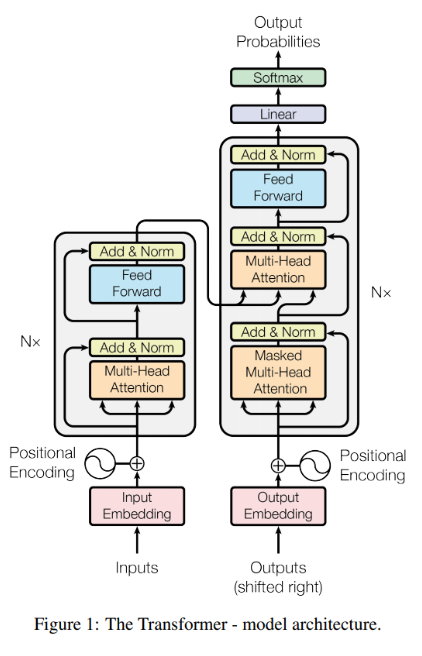
\includegraphics[width=0.35\linewidth]{transformer.png}
\caption{Model architecture of the transformer}
\label{transformer}
\end{figure}
\begin{enumerate}[label=(\alph*)]

    \item Implement \texttt{attention} function in \texttt{BertSelfAttention} class of \texttt{bert.py}. Scaled dot-product attention are computed as below: 
        \begin{align}
\text{Attention}(Q,K,V) = \text{softmax}(\frac{QK^T}{\sqrt{d_k}})V
\end{align} \textbf{(10 pts)}
    \item Implement \texttt{forward} function in \texttt{BertSelfAttention} class of \texttt{bert.py}. \textbf{(8 pts)}
    \item Implement \texttt{add\_norm} function in \texttt{BertLayer} class of \texttt{bert.py}. It corresponds to Add \& Norm Layer in the figure \ref{transformer}, which is defined as $\text{LayerNorm}(x+\text{Sublayer}(x))$ \textbf{(8 pts)}

    \item  Implement \texttt{forward} function in \texttt{BertLayer} class of \texttt{bert.py}. It corresponds to encoder stacks which are described on the left of the figure \ref{transformer}. After completing the codes, run \texttt{python sanity\_check.py} to check your implementation. \textbf{(8 pts)}
  \item  Implement \texttt{train} function in \texttt{classifier.py}. This function carries out backpropagation through the model parameters. \textbf{(8 pts)}
  
   \item Show time! Run \texttt{sbatch run.sh}. Each time you run the above code, a \texttt{'result.log'} file is created (be cautious as it overwrites the existing one). When submitting, make sure to attach the \texttt{'result.log'} file as well. \textbf{You don't need to submit the model checkpoint (.pt file) and *-output.txt files.} \textbf{(8 pts)} 
\end{enumerate}

\end{document}
